\chapter{K"unstliche neuronale Netze}
{
K"unstliche Intelligenz l"asst sich mit einem K"unstlichen Neuronalen Netz (KNN) realisieren. KNNs basieren auf dem Vorbild des biologischen neuronalen Netz des Gehirns.
\cite{Breitner} schreibt dazu:
\begin{quote}{\glqq}Die biologischen Vorg"ange des menschlichen Denkens und Lernens (Aktivierung von Neuronen, chemische Ver"anderung von Synapsen usw.) werden, so gut wie m"oglich, mathematisch beschrieben und in Software oder Hardware modelliert.{\grqq}\end{quote}
KNNs bestehen also aus einem Satz von Algorithmen, welche Daten interpretieren. Diese Eingangsdaten sind numerisch und m"ussen meist durch Umwandlung der originalen Daten (z.B. Bilder, Text oder Musik) geschaffen werden. Sie sind dazu entwickelt anhand von Mustererkennung Daten eigenst"andig zu Gruppieren, vorgegebenen Klassen zu zuordnen oder den weiteren Verlauf vorherzusagen.

Das Training eines KNNs l"asst sich in zwei Kategorien unterteilen: das "uberwachte Lernen und das un"uberwachte Lernen. Beim "uberwachten lernen werden dem Netz Eingangs- und Ausgangsdaten gegeben anhand dessen das Netz den Zusammenhang erlernt und sp"ater in der Lage ist neue Daten entsprechend zu klassifizieren oder die n"achsten Ausgabe vorherzusagen. Beim un"uberwachten Lernen erh"alt das Netz lediglich Eingangsdaten und lernt diese anhand von "Ahnlichkeiten  zu gruppieren.

Es gibt verschiedene Arten von K"unstlichen Neuronalen Netzen und in den folgenden Abschnitten werden drei von ihnen erkl"art.


\section{Feedforward Netzwerke}
Ein Feedforward Netzwerk besteht aus Layern und Neuronen. Die Neuronen sind f"ur die Berechnungen der Ausgabe zust"andig, w"ahrend die Layer den Aufbau des Netzes bestimmen. Abbildung 2.1 zeigt einen m"oglichen Aufbau eines k"unstliches Neurons.
\renewcommand{\figurename}{Abb.}
\begin{figure}[htp]
\centering
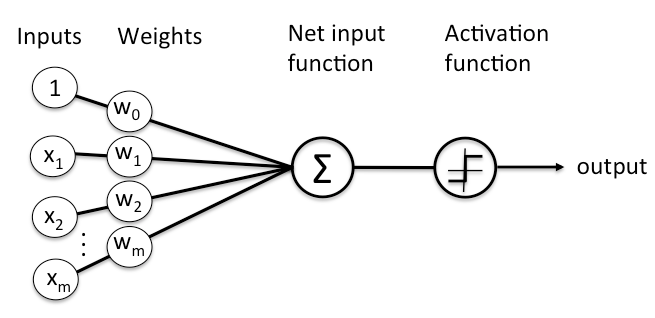
\includegraphics[width=0.60\textwidth]{pictures/perceptron_node.png}
\caption[Feedforward Neuron]{m"ogliches Aussehen eines Feedforward Neurons (Quelle: \cite{DL4Jimg1})}
\end{figure}
Dieses Neuron besteht aus 1 bis x\textsubscript{m} Eing"angen (Inputs) mit Gewichten (Weights), einer Eingangsfunktion (Net input function), einer Aktivierungsfunktion (Activation function) und einem Ausgang (Outputs). Die zu verarbeiteten Daten werden an die Eing"ange gelegt, durch die zugeh"origen Gewichte verst"arkt oder abgeschw"acht und anschlie{\ss}end durch die Eingangsfunktion aufsummiert. Die entstandene Summe wird dann an die Aktivierungsfunktion "ubergeben, welche das Ergebnis dieses Neurons festlegt.

Ein Layer besteht aus einer Reihe von Neuronen beliebiger Anzahl. Ein k"unstliches neuronales Netz setze sich aus einem Input Layer, einem Output Layer und beliebig vielen Hidden Layern zusammen. Hat ein Netz mehr als ein Hidden Layer so wird es auch als Deep Learning Netz bezeichnet.
\renewcommand{\figurename}{Abb.}
\begin{figure}[htp]
\centering
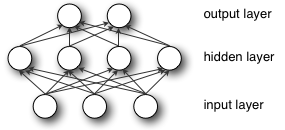
\includegraphics[width=0.50\textwidth]{pictures/mlp.png}
\caption[Aufbau eines Feedforward Netzes]{Aufbau eines Feedforward Netzes (Quelle: \cite{DL4Jimg1})} 
\end{figure}
Abbildung 2.2 zeigt ein Feedforward Netzwerk. Bei diesem Netz besitzt das Input Layer drei Neuronen, das Hidden Layer hat vier und das Output Layer hat zwei Neuronen. Die Ergebnisse des Input und Hidden Layers dienen dem nachfolgenden Layer als Eingang. Die Eing"ange des Input Layers und der Ausgang des Output Layers sind hier nicht dargestellt, da der Fokus auf der inneren Verkn"upfung liegen soll. Jedes Neuron hat hier so viel Ausg"ange wie die Anzahl der Neuronen im folgenden Layer und ist somit vollst"andig verkn"upft. Dies muss nicht immer der Fall sein, doch auf diesen Sonderfall soll hier nicht weiter eingegangen werden.


\subsection{Training durch Backpropagation}
Ein neuronales Netz kann anhand von Trainingsdaten eine Funktion erlernen, indem es die Gewichte ver"andert. Um sinnvolle Ergebnisse zu erhalten m"ussen die Gewichte solange angepasst werden, bis der Fehler zwischen Netzausgabe und tats"achlichen Ausgabewert am kleinsten ist. Dies wird mit Hilfe der Backpropagation gemacht, indem R"uckw"arts vom Fehler "uber die Ausg"ange, die Gewichte und die Eing"ange der verschiedenen Layer ein Zusammenhang zwischen Fehlergr"o{\ss}e und einzelnen Gewichtseinstellungen hergestellt wird. F"ur die Bestimmung der ben"otigten Gewichten benutzt man Optimierungsfunktionen. Eine weitverbreitete Optimierungsfunktion hei{\ss}t Gradient Descent. Sie beschreibt das Verh"altnis des Fehlers zu einem einzelnen Gewicht und wie sich der Fehler ver"andert wenn das Gewicht angepasst wird.

Das Ziel ist m"oglichst schnell den Punkt zu erreichen an dem der Fehler am kleinsten ist. Um dies zu erreichen wiederholt das Netz so oft wie n"otig die folgenden Schritte: Ergebnis anhand der aktuellen Gewichte bestimmen, Fehler messen, Gewichte aktualisieren.


\section{Recurrent Netzwerke}
Recurrent Neuronal Networks (RNN) betrachten im Gegensatz zu Feedforward Netzwerken nicht nur die aktuellen Eingangsdaten sondern auch die vorhergegangenen. Sie besitzen daher zwei Eingangsgr"o{\ss}en, n"amlich die gerade angelegten und die zur"uckgeleiteten aus dem vorherigen Zeitschritt.
\renewcommand{\figurename}{Abb.}
\begin{figure}[htp]
%%\begin{floatingfigure}[r]{textwidth}
\centering
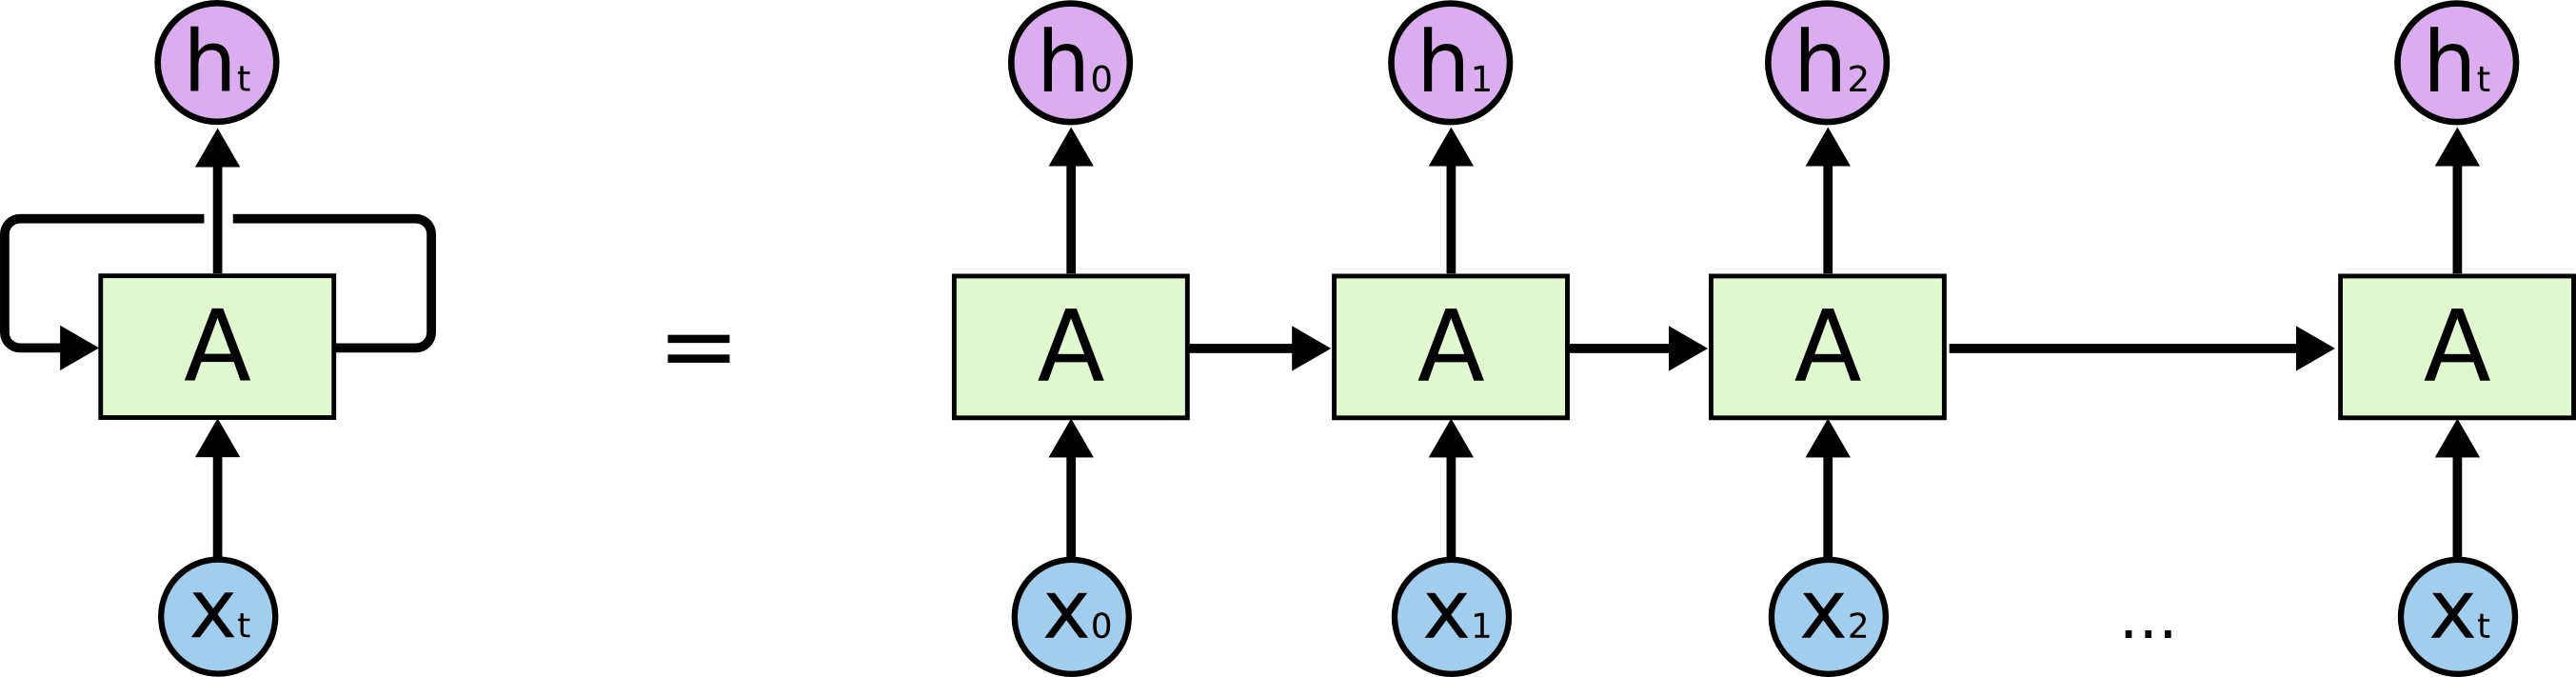
\includegraphics[width=0.60\textwidth]{pictures/RNN-unrolled.png}
\caption[RNN Neuron]{vereinfachte Darstellung eines RNN Neurons (Quelle: \cite{OlahImg})}
%%\end{floatingfigure} 
\end{figure}
Abbildung 2.3 zeigt links eine vereinfachte Darstellung eines RNN Neurons mit R"uckf"uhrung, aber ohne dargestellte Gewichte oder Aktivierungsfunktion. Rechts ist das Ganze als zeitlicher Verlauf dargestellt. Im ersten Zeitschritt wird x\textsubscript{0} an den Eingang gelegt und h\textsubscript{0} als Ergebnis berechnet. Au{\ss}erdem f"uhrt ein Pfeil zum Neuron im zweiten Zeitschritt und dient dort als zweiter Eingang. Das Ergebnis, das ein Neuron liefert ist also immer vom vorherigen abh"angig. Man bezeichnet dies auch als Ged"achtnis des Netzes. Einem Netz ein Ged"achtnis zu geben macht immer dann Sinn, wenn die Eingangsdaten eine Sequenz bilden und nicht komplett unabh"angig von einander sind. Im Gegensatz zu den Feedforward Netzen k"onnen Recurrent Netzwerke Sequenzen erfassen und sie zur Erzeugung ihrer Ausgaben nutzen. Dies ist zum Beispiel bei der automatischen Textgenerierung hilfreich, wo ein folgender Buchstabe immer vom vorherigen abh"angt und nicht willk"urlich gew"ahlt werden kann. Ein RNN ist in der Lage gezielt auf ein q ein u folgen zu lassen um sinnvolle W"orter zu bilden, ein Feedforward Netzwerk kann das nicht.

\subsection{Training durch Backpropagation Through Time}
Da bei Recurrent Netzen das Ergebnis und somit der Fehler nicht nur vom aktuellen Zeitschritt abh"angt, muss auch die Backpropagation erweitert werden um sinnvoll arbeiten zu k"onnen. Backpropagation Through Time (BPTT) erg"anzt die normale Backpropagation um den Faktor Zeit, so dass ein Einfluss auf den Fehler von einem Gewicht aus fr"uheren Schritten ermittelt werden kann. Abbildung 2.4 soll diesen Vorgang verdeutlichen. 
\renewcommand{\figurename}{Abb.}
\begin{figure}[hb]
\centering
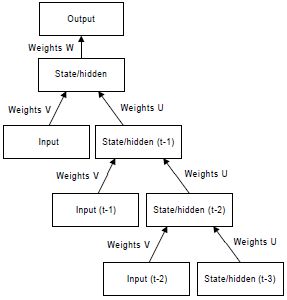
\includegraphics[width=0.65\textwidth]{pictures/bptt_cut.png}
\caption[BPTT]{entrolltes RNN f"ur BPTT (Quelle: \cite{BPTT})}
\end{figure}
Sie zeigt ein Recurrent Netz das um drei Zeitschritte entrollt wurde indem Komponenten dupliziert wurden. Dadurch l"osen sich die R"uckf"uhrungen auf und das Netzwerk verh"alt sich wie ein Feedforward Netz. Der Einfluss jedes Gewichts kann nun anteilig berechnet und anschlie{\ss}end summiert werden, so dass ein einzelner Wert je Gewicht f"ur die Anpassung ermittelt wird.

Dieses Verfahren ben"otigt nat"urlich mehr Speicher, da alle vorherigen Zust"ande und Daten f"ur eine bestimme Anzahl an Zeitschritten gespeichert werden m"ussen.


\subsection{Problem der verschwindenden und explodierenden Gradienten}
Der Gradient stellt die Ver"anderung aller Gewichte in Bezug auf Ver"anderung im Fehler dar. Wenn der Gradient unbekannt ist, ist eine Ver"anderung an den Gewichten zur Verkleinerung des Fehlers nicht m"oglich und das Netz ist nicht in der Lage zu lernen. Zu unbekannten Gradienten kann es kommen, da Informationen die durch ein Deep Netz flie{\ss}en vielfach multipliziert werden. Multipliziert man einen Betrag regelm"a{\ss}ig mit einem Wert knapp gr"o{\ss}er 1 kann das Ergebnis unmessbar gro{\ss} werde und in diesem Fall spricht man von einem explodierenden Gradienten. Umgekehrt f"uhrt eine wiederholte Multiplikation eines Betrages mit einem Wert kleiner als 1 zu einem sehr kleinem Ergebnis. Der Wert kann so klein werden, dass er von einem Netz nicht mehr gelernt werden kann. Hier spricht man von einem verschwindenden Gradienten.

Das Problem der explodierenden Gradienten l"asst sich durch eine sinnvolle Obergrenze beheben. Bei den verschwindenden Gradienten sieht eine L"osung wesentlich schwieriger aus und dieses Thema ist noch immer Gegenstand der Forschung.


\subsection{Problem der Langzeit-Abh"angigkeiten}
Wie bereits erw"ahnt sind RNNs in der Lage Sequenzen zu erkennen und mit Abh"angigkeiten zu arbeiten, doch diese F"ahigkeit ist leider begrenzt. Besteht nur eine kleine zeitliche L"ucke zwischen den von einander abh"angigen Daten, ist ein RNN in der Lage diesen Zusammenhang zu erkennen und die richtigen Schl"usse zu ziehen. Wird der zeitliche Abstand zwischen Eingabe der Daten und dem Zeitpunkt an dem sie f"ur ein Ergebnis ben"otigt werden jedoch sehr gro{\ss} kann ein RNN diesen Zusammenhang nicht mehr herstellen. Als Beispiel gibt \cite{Olah} in seinem Artikel ein Sprach-Model an, welches das n"achste Wort abh"angig vom Vorherigen vorhersagt. Ein RNN ist in der Lage im Satz {\glqq}Die Wolken sind im Himmel.{\grqq} das letzte Wort vorauszusagen, da der Abstand von Himmel und Wolken sehr klein ist. Im Text {\glqq}Ich bin in Frankreich aufgewachsen. ... Ich spreche flie{\ss}end franz"osisch.{\grqq} kann der Abstand zum letzten Wort aber sehr gro{\ss} sein und die vorherigen W"orter lassen lediglich den Schluss zu das eine Sprache folgen muss. Denn Kontext, dass es sich sehr wahrscheinlich um franz"osisch handelt, erh"alt man nur durch den ersten Satz. Ein RNN kann sich aber keinen ganzen Text merken und somit hier den Zusammenhang von Frankreich und franz"osisch nicht lernen.

Um das Problem der Langzeit-Abh"angigkeiten zu l"osen, benutzt man Long Short-Term Memory Netze.


\section{Long Short-Term Memory Netze}
Long Short-Term Memory (LSTM) Netze sind eine besondere Art von Recurrent Netzwerken, die mit Langzeit-Abh"angigkeiten arbeiten k"onnen. Sie wurden so entworfen, dass sie speziell dieses Problem l"osen, denn Informationen "uber einen langen Zeitraum zu speichern ist ihr Standardverhalten und nicht etwas was m"uhsam erlernt werden muss. Sie bestehen aus Speicherzellen, in die Informationen geschrieben und wieder herausgelesen werden k"onnen. Mit Hilfe von sogenannten Gates, die ge"offnet oder geschlossen werden, entscheidet eine Zelle was gespeichert wird und wann ein Auslesen, Reinschreiben und L"oschen erlaubt ist. Diese Gates sind analog und durch eine Sigmoid-Funktion implementiert, so dass sich ein Bereich von 0 bis 1 ergibt. (Analog hat den Vorteil gegen"uber digital dass es differenzierbar ist und somit f"ur die Backpropagation geeignet.)
\renewcommand{\figurename}{Abb.}
\begin{figure}[htb]
\centering
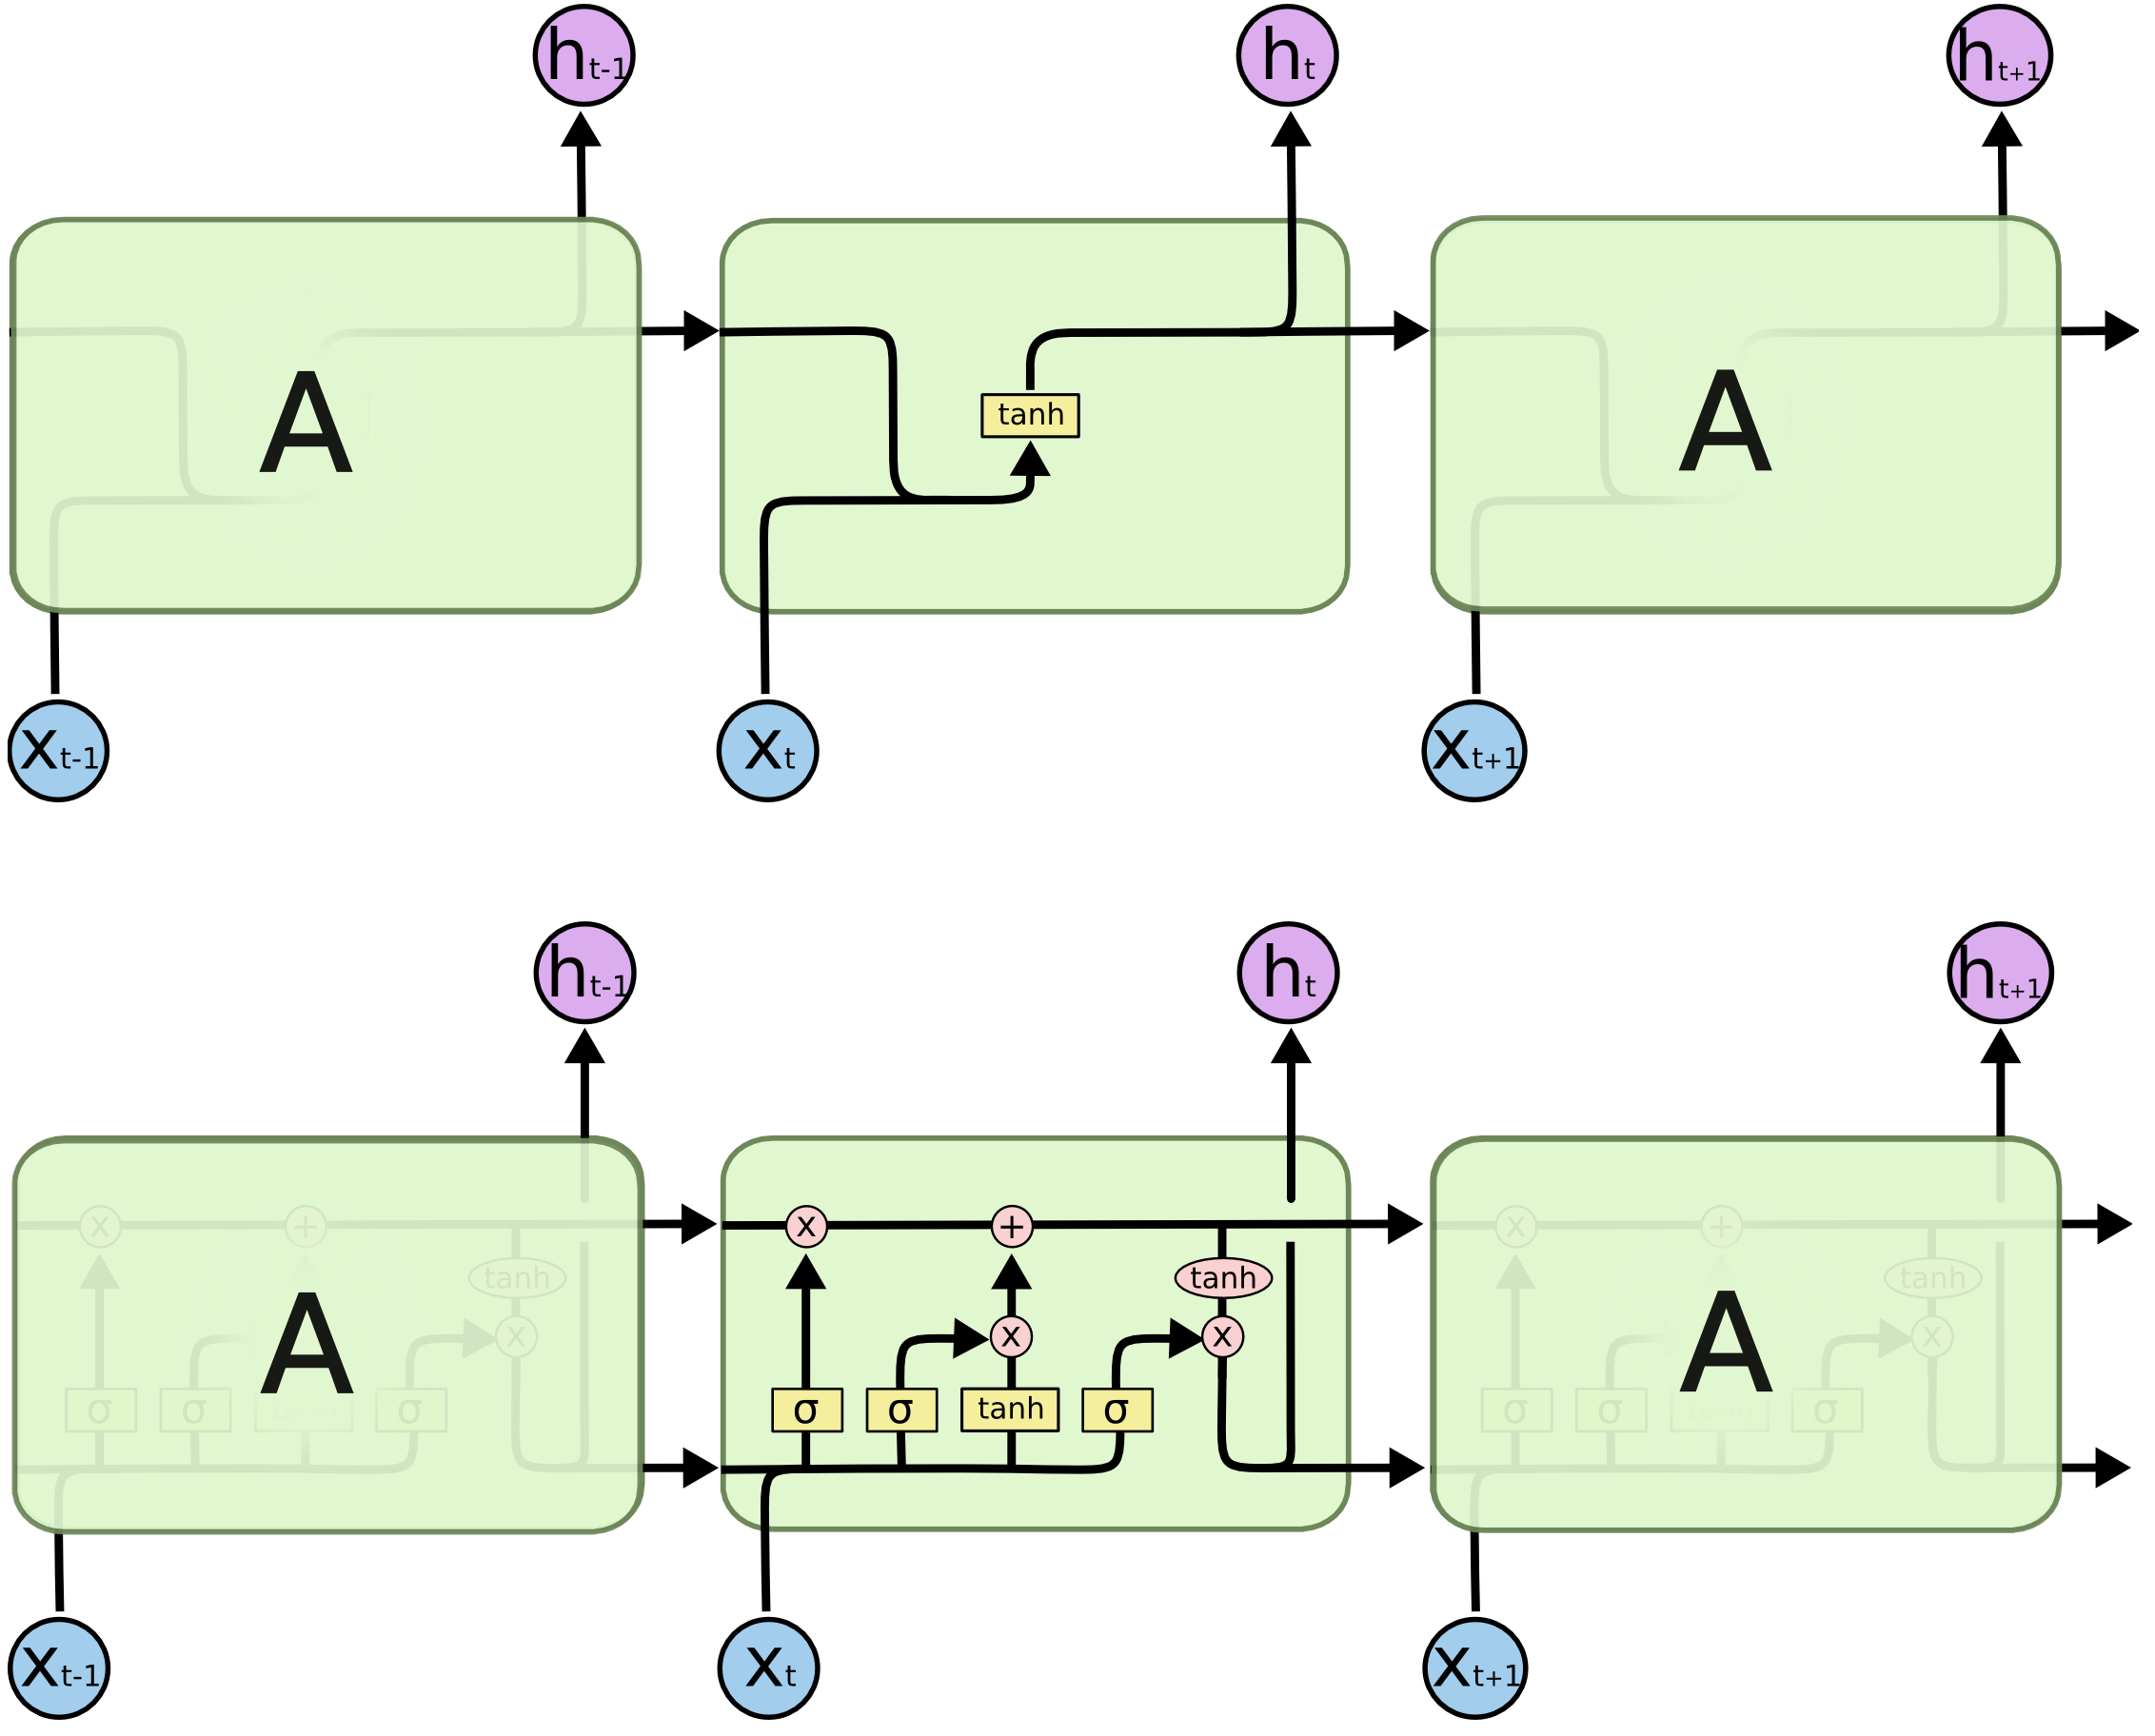
\includegraphics[width=0.75\textwidth]{pictures/SRN-LSTM-chain.png}
\caption[Vergleich RNN und LSTM]{Vergleich RNN und LSTM (Quelle: \cite{OlahImg})}
\end{figure}
Genau wie die Eing"ange bei den Feedforward und Recurrent Netzen besitzen die Gates Gewichte. Diese Gewichte werden ebenfalls w"ahrend des Lernprozesses angepasst, so dass die Zelle lernt wann Daten eingelassen, ausgelesen oder gel"oscht werden m"ussen.

Abbildung 2.5 zeigt zum Vergleich oben ein simples Recurrent Netz und unten ein LSTM Netz. Beide sind "uber drei Zeitschritte dargestellt, wobei der zweite Schritt jeweils ihr Innenleben wiedergibt. W"ahrend beim RNN eine simple Struktur mit nur einer Funktion (gelber Kasten in der Abbildung) f"ur das Ergebnis verantwortlich ist, benutzt ein LSTM vier Funktionen. Wie diese Funktionen mit einander agieren und zu einem Ergebnis kommen wird im n"achsten Abschnitt Schrittweise erkl"art.


\subsection{Aufbau einer Speicherzelle}
\subsubsection{Zellzustand}
\begin{wrapfigure}{r}{0.45\textwidth}
  \vspace{-30pt}
  \begin{center}
    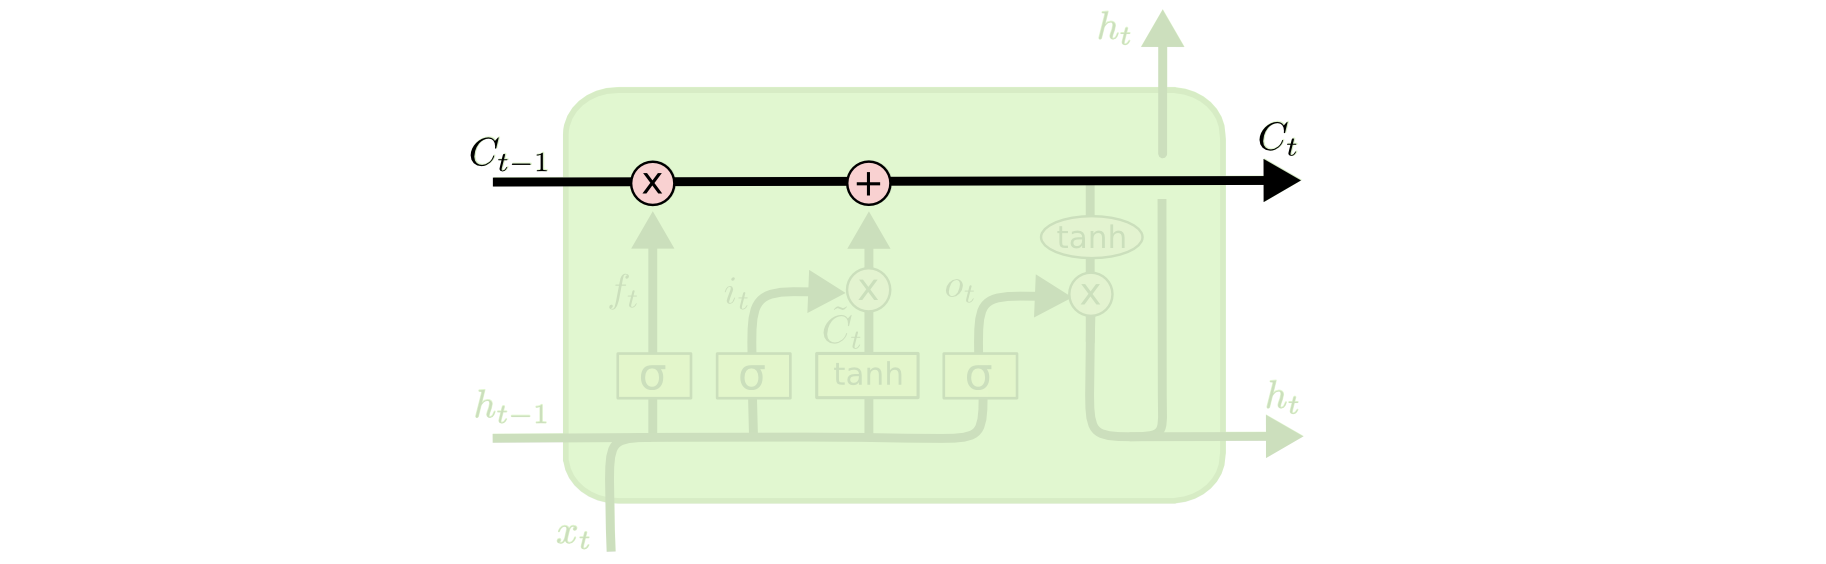
\includegraphics[width=0.45\textwidth]{pictures/LSTM3-C-line.png}
  \end{center}
  \vspace{-20pt}
  \caption[LSTM Zellzustand]{LSTM Zellzustand (Quelle: \cite{OlahImg})}
\vspace{-10pt}
\end{wrapfigure}
Der Zellzustand ist der eigentliche Speicherort oder das Ged"achtnis des LSTM. Abbildung 2.6 zeigt den Verlauf durch eine Speicherzelle. Links wird der Zellzustand vom vorherigen Zeitschritt "ubernommen und rechts an den n"achsten weitergegeben. In der Mitte sind zwei Operation, die den Zustand w"ahrend dieses Zeitschrittes ver"andern k"onnen. Welche Aufgabe sie haben folgt im Abschnitt Zellzustands Update.

\subsubsection{Forget Gate}
\begin{wrapfigure}{r}{0.45\textwidth}
  \vspace{-30pt}
  \begin{center}
    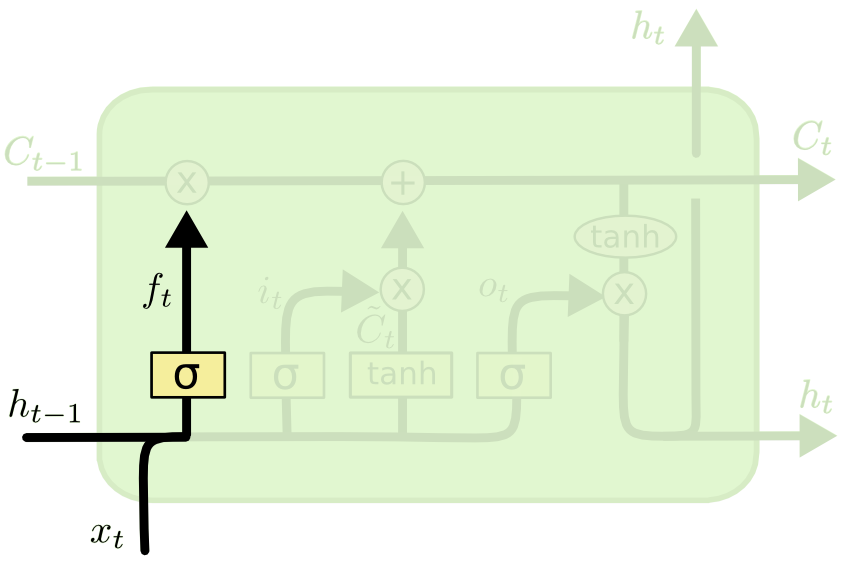
\includegraphics[width=0.45\textwidth]{pictures/LSTM3-focus-f_cut.png}
  \end{center}
  \vspace{-20pt}
  \caption[LSTM: Forget Gate]{Forget Gate (Quelle: \cite{OlahImg})}
\vspace{-10pt}
\end{wrapfigure}
Das Forget Gate entscheidet mit Hilfe der Sigmoid-Funktion welche Informationen gel"oscht werden. Es sieht sich den alten Ausgang h\textsubscript{t-1} und den neuen Eingang x\textsubscript{t} an und gibt f"ur jede Information im Zellzustand C\textsubscript{t-1} einen Wert zwischen 0 und 1 an. Eine 1 bedeutet behalte es und eine 0 vergiss bzw. l"osche es.

Der Grund f"ur das Vorhandensein einer Vergissfunktion in einem Baustein, der die Aufgabe hat sich Sachen zu merken, liegt darin dass es manchmal sinnvoll sein kann Dinge zu vergessen. Zum Beispiel kann mit ihrer Hilfe die Speicherzelle zur"uckgesetzt werden, wenn bekannt ist dass die folgenden Daten in keinem Zusammenhang zu den vorherigen stehen.

\subsubsection{Eingang}
\begin{wrapfigure}{r}{0.45\textwidth}
  \vspace{-30pt}
  \begin{center}
    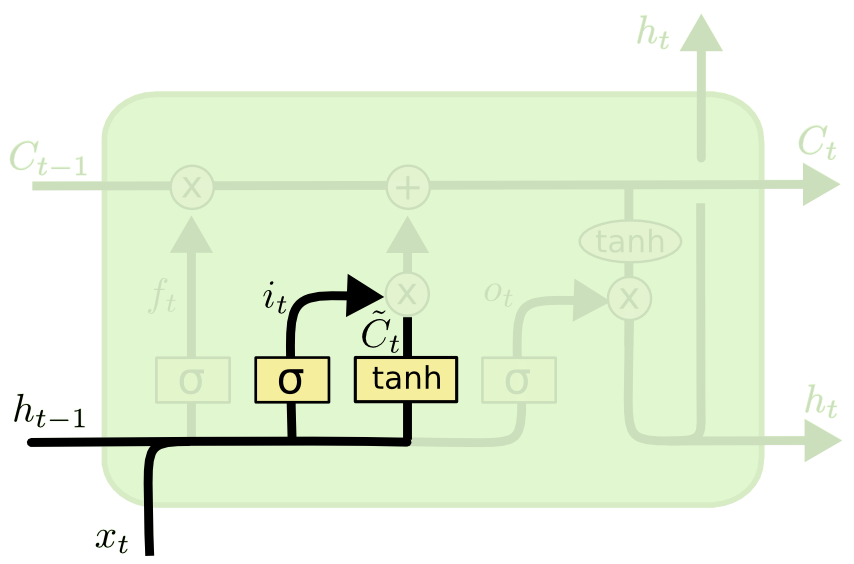
\includegraphics[width=0.45\textwidth]{pictures/LSTM3-focus-i_cut.png}
  \end{center}
  \vspace{-20pt}
  \caption[LSTM: Eingangsgate]{Eingangsgate (Quelle: \cite{OlahImg})}
\vspace{-10pt}
\end{wrapfigure}
Die Entscheidung, welche Daten gespeichert werden sollen, besteht aus zwei Teilen. Das Eingangsgate ist ebenfalls eine Sigmoid-Funktion und liefert ein Ergebnis zwischen 0 und 1. Sie entscheidet welche Daten zum Zellzustand wie stark durchgelassen werden. Au{\ss}erdem bereitet eine tanh-Funktion die Daten so auf, dass sie im Zellzustand gespeichert werden k"onnen.

\subsubsection{Zellzustands Update}
\begin{wrapfigure}{r}{0.45\textwidth}
  \vspace{-30pt}
  \begin{center}
    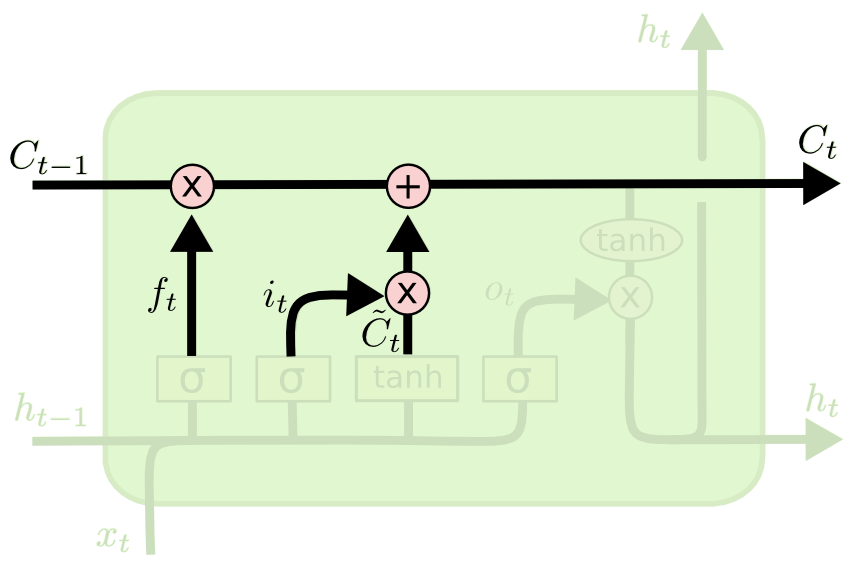
\includegraphics[width=0.45\textwidth]{pictures/LSTM3-focus-C_cut.png}
  \end{center}
  \vspace{-20pt}
  \caption[LSTM: Zellzustands Update]{Zellzustands Update (Quelle: \cite{OlahImg})}
\vspace{-10pt}
\end{wrapfigure}
Nachdem das Forget Gate und das Eingangsgate entschieden haben was mit den Daten passieren soll, wird der Zellzustand aktualisiert. Daf"ur wird der alte Zellzustand C\textsubscript{t-1} mit dem Ergebnis f\textsubscript{t} des Forget Gates multipliziert und somit alles gel"oscht, das vergessen werden soll. Anschlie{\ss}end werden die vom Eingangsgate skalierten und von der tanh-Funktion vorbereiteten Daten zum Zellzustand addiert.

\subsubsection{Ausgabe}
\begin{wrapfigure}{r}{0.45\textwidth}
  \vspace{-30pt}
  \begin{center}
    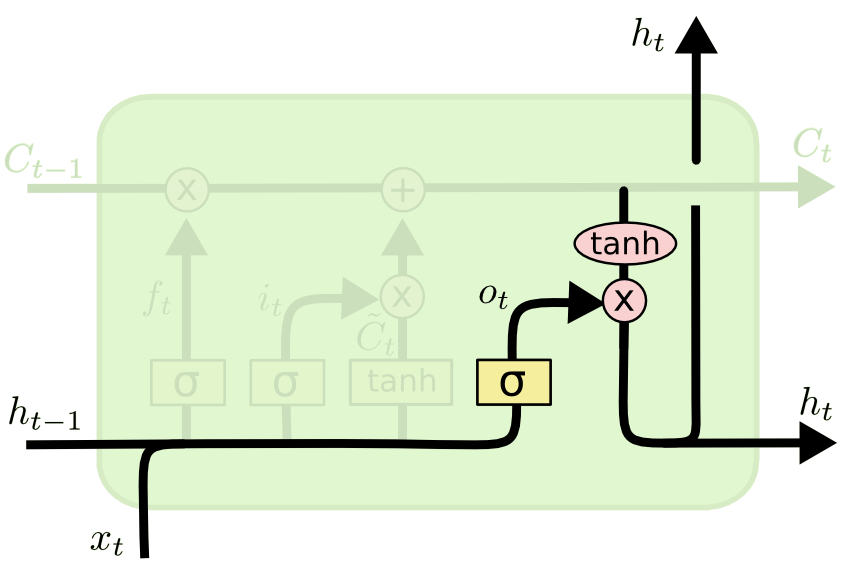
\includegraphics[width=0.45\textwidth]{pictures/LSTM3-focus-o_cut.png}
  \end{center}
  \vspace{-20pt}
  \caption[LSTM: Ausgabe]{Ausgabe (Quelle: \cite{OlahImg})}
\vspace{-10pt}
\end{wrapfigure}
Die Ausgabe erfolgt mit Hilfe eines Ausgabegates, welches ebenfalls eine Sigmoid-Funktion ist. Der Zellzustand wird durch eine tanh-Funktion geleitet und anschlie{\ss}end mit dem Ergebnis der Sigmoid-Funktion multipliziert. Die tanh-Funktion wandelt die Werte in einen Bereich von -1 bis 1 um, welches der typische Wertebereich von KNN-Ausg"angen ist. Durch die Multiplikation kontrolliert das Ausgangsgate, ob und wie stark das Ergebnis ausgegeben wird.

\subsubsection{Zusammenfassung}
Eine Speicherstelle besteht aus einem Zellzustand, der als Ged"achtnis fungiert und drei Gates, die den Zellzustand besch"utzen und kontrollieren. Jedes Gate arbeitet mit einer Sigmoid-Funktion, die einen Wertebereich zwischen 0 und 1 ausgibt und damit die Itensit"at der Aktion bestimmt. Das Forget Gate ist f"ur das L"oschen zust"andig, das Eingangsgate "ubernimmt die Aktion das Neu-Merkens indem es neue Informationen in den Zellzustand speichert und das Ausgangsgate bestimmt die Informationen die ausgegeben werden.


\subsection{LSTM Varianten}
Nicht alle LSTM sind so aufgebaut wie bisher beschrieben. Es gibt viele durch kleine Ver"anderungen leicht abweichende Versionen. Da eine komplette Auflistung den Umfang dieser Arbeit sprengen w"urden, werden hier nur zwei Varianten vorgestellt um einen Eindruck zu vermitteln, welche M"oglichkeiten es gibt.

\subsubsection{Guckl"ocher}
\begin{wrapfigure}{r}{0.35\textwidth}
  \vspace{-40pt}
  \begin{center}
    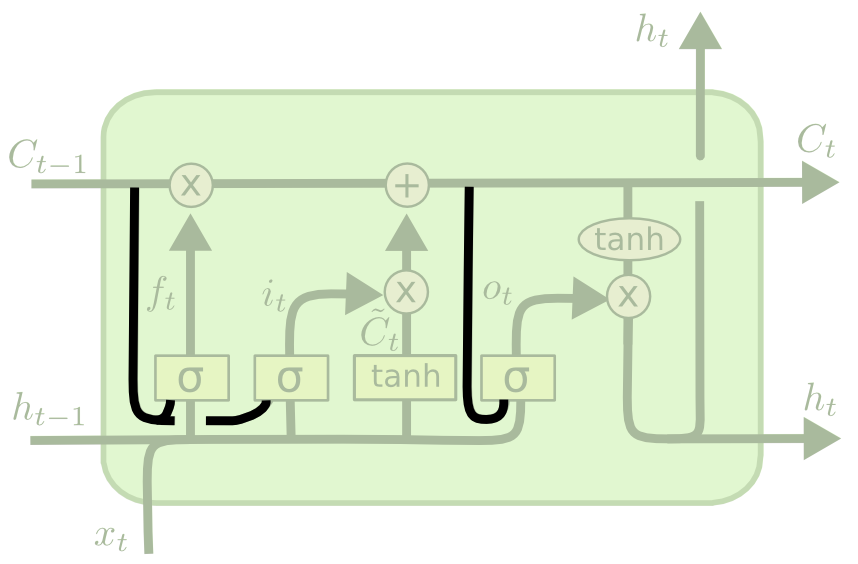
\includegraphics[width=0.35\textwidth]{pictures/LSTM3-var-peepholes_cut.png}
  \end{center}
  \vspace{-20pt}
  \caption[LSTM Variante: Guckl"ocher]{Variante Guckl"ocher (Quelle: \cite{OlahImg})}
\vspace{-10pt}
\end{wrapfigure}
In dieser Variante werden den Gates eine Guckloch-Verbindung hinzugef"ugt. Dies erm"oglicht es den Gates einen Einblick in den aktuellen Zellzustand zu nehmen und die dadurch gewonnenen Informationen in ihre Entscheidung einflie{\ss}en zu lassen. Abbildung 2.11 zeigt diese Verbindungen f"ur alle drei Gates, jedoch ist dies nicht zwingend notwendig. Es besteht die M"oglichkeit auch nur einem oder zwei Gates diese Verbindung zu geben.

\subsubsection{Zusammengef"uhrte Gates}
\begin{wrapfigure}{r}{0.35\textwidth}
  \vspace{-40pt}
  \begin{center}
    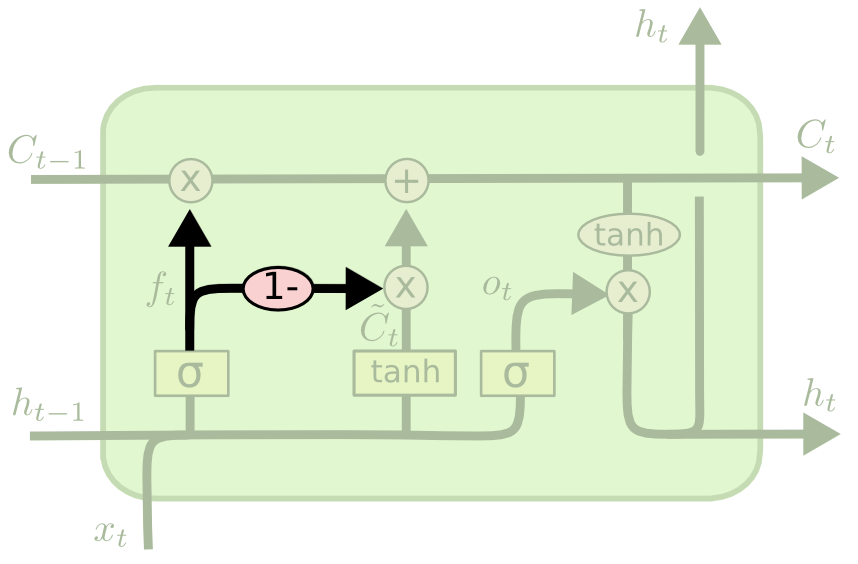
\includegraphics[width=0.35\textwidth]{pictures/LSTM3-var-tied_cut.png}
  \end{center}
  \vspace{-20pt}
  \caption[LSTM Variante: Zusammengef"uhrte Gates]{Variante Zusammengef"uhrte Gates (Quelle: \cite{OlahImg})}
\vspace{-10pt}
\end{wrapfigure}
Eine andere Variante ist in Abbildung 2.12 dargestellt und schlie{\ss}t das Forget Gate und das Eingangsgate zu einem Gate zusammen. Diese Ver"anderung hat die Auswirkung, dass die Entscheidung was gel"oscht und was neu gespeichert wird nur noch gemeinsam getroffen werden kann. Somit kann nur etwas vergessen werden, wenn es durch neue Informationen ersetzt wird und im Umkehrschluss k"onnen neue Informationen nur gespeichert werden, wenn andere Informationen aus dem Zellzustand gel"oscht werden.


\section{Aktueller Forschungsstand (unfinished)}

\subsection{noch ohne Titel}

\subsubsection{Analyse von LSTM-Netz-Varianten (LSTM: A Search Space Odyssey)}
- In recent years, these networks have become the state-of-the-art models for a variety of machine learning problems.
- In this paper, we present the first large-scale analysis of eight LSTM variants on three representative tasks: speech recognition, handwriting recognition, and polyphonic music modeling.
- In total, we summarize the results of 5400 experimental runs (~15 years of CPU time), which makes our study the largest of its kind on LSTM networks.
- Our results show that none of the variants can improve upon the standard LSTM architecture significantly, and demonstrate the forget gate and the output activation function to be its most critical components.
- The focus of our study is to compare different LSTM variants, and not to achieve state-of-the-art results. Therefore, our experiments are designed to keep the setup simple and the comparisons fair. The vanilla LSTM is used as a baseline and evaluated together with eight of its variants. Each variant adds, removes or modifies the baseline in exactly one aspect, which allows to isolate their effect. Three different datasets from different domains are used to account for cross-domain variations.
Quelle: 1503.04069v1.pdf

\subsubsection{Bedienung dynamischer Systeme (Control of Dynamic Systems Using LSTM supported Neural Network)}
- operation of dynamic system is challenged by non-linearity, disturbances and multivariate interactions
	- well-suited for to handle this is MPC
- combination of LSTM and NN(Neural Network) to learn complex policies of MPC(Model Predictive Control)
- MPC is a multivariate control algorithm that uses an internal dynamic model of the process, history of past control moves to yield optimal control actions.
	- In MPC, the control actions are computed by solving an optimization objective that minimizes a cost function ( function of difference in target output and system output) while accounting for system dynamics ( using a prediction model) and satisfying output and control action constraints.
	- However, solving the optimization objective in real time is computationally demanding and often takes lot of time for complex systems. Moreover, MPC requires the estimation of hidden system states (hidden states characterize system dynamics) which can be challenging in complex non-linear dynamic system.
- We propose LSTM supported NN model (LSTMSNN). The output of LSTMSNN is a weighted combination of outputs from LSTM and NN. We use this combination because the current control action depends on past control actions, current system output and target output. The LSTM part of LSTMSNN takes past control actions as input. Because there is temporal dependency between control actions, and we want to use LSTM to capture it. The NN part of LSTMSNN takes current system output and target output as input. Because we want to train NN to make a decision on control action by using current system and target output.
	- Our trained LSTMSNN Model is computationally less expensive than MPC.
	- Moreover, our approach does not involve the burden of estimating the hidden states that characterizes system dynamics.
Quelle: 2\_lstmsnn.pdf

\subsubsection{LSTM-Netzwerk-basierte Merkmalextraktion (LSTM Networks for Mobile Human Activity Recognition)}
- In this paper, we propose a LSTM-based feature extraction approach to recognize human activities using tri-axial accelerometers data.
- The predominant approach to HAR is based on a sliding window procedure, where a fixed length analysis window is shifted along the signal sequence for frame extraction. Preprocessing then transforms raw signal data into feature vectors, which are subjected to statistical classifiers that eventually provide activity hypotheses.
- Activity recognition has a wide range of applications in mobile applications — from fitness and health tracking to context-based advertising and employee monitoring.
- The features used in most of researches on HAR are selected by hand. Designing hand-crafted features in a specific application requires domain knowledge [18], and maybe result in loss of information after extracting features.
Quelle: 014.pdf

\subsubsection{Semantically Conditioned LSTM-based Natural Language Generation for Spoken Dialogue Systems}
- This paper presents a statistical language generator based on a semantically controlled Long Short-term Memory (LSTM) structure. The LSTM generator can learn from unaligned data by jointly optimising sentence planning and surface realisation using a simple cross entropy training criterion, and language variation can be easily achieved by sampling from output candidates. With fewer heuristics, an objective evaluation in two differing test domains showed the proposed method improved performance compared to previous methods. Human judges scored the LSTM system higher on informativeness and naturalness and overall preferred it to the other systems.
- The most common and widely adopted today is the rule-based (or template-based) approach (Cheyer and Guzzoni, 2007; Mirkovic and Cavedon, 2011). Despite its robustness and adequacy, the frequent repetition of identical, rather stilted, output forms make talking to a rule-based generator rather tedious.
Quelle: 1508.01745v2.pdf

\subsection{Musikerzeugung}

\subsubsection{Modelling High-Dimensional Sequences with LSTM-RTRBM: Application to Polyphonic Music Generation}
- We propose an automatic music generation demo based on artificial neural networks, which integrates the ability of Long Short-Term Memory (LSTM) in memorizing and retrieving useful history information, together with the advantage of Restricted Boltzmann Machine (RBM) in high dimensional data modelling. Our model can generalize to different musical styles and generate polyphonic music better than previous models.
- In this context, we wish to combine the ability of RBM to represent a complicated distribution for each time step, together with a temporal model in sequence. We consider both long-term memory and short-term memory in our design of guide and learning modules, by increasing a bypassing channel from data source filtered by a recurrent LSTM layer and we show that our model increases performance generally.
Quelle: 582.pdf

\subsubsection{Polyphonic Music Modelling with LSTM-RTRBM}
- Our model integrates the ability of Long Short-Term Memory (LSTM) in memorizing and retrieving useful history information, together with the advantage of Restricted Boltzmann Machine (RBM) in high dimensional data modelling. Our approach greatly improves the performance of polyphonic music sequence modelling, achieving the state-of-the-art results on multiple datasets.
- For example, in order to complete a melody line, the beginning of the music sequence needs to be held in mind while the rest is played, a task which is carried out by the short-term memory. And the long-term memory will serve as the theme and emotion that will help maintain the global coherence of music. The existence of both the short-term and the longterm memory is vital for generating melodic and coherent music sequences.
Quelle: p991-lyu.pdf





https://colah.github.io/posts/2015-08-Understanding-LSTMs/
LSTMs were a big step in what we can accomplish with RNNs. It’s natural to wonder: is there another big step? A common opinion among researchers is: "Yes! There is a next step and it’s attention!" The idea is to let every step of an RNN pick information to look at from some larger collection of information. For example, if you are using an RNN to create a caption describing an image, it might pick a part of the image to look at for every word it outputs. In fact, Xu, et al. (2015) do exactly this – it might be a fun starting point if you want to explore attention! There’s been a number of really exciting results using attention, and it seems like a lot more are around the corner…
Attention isn’t the only exciting thread in RNN research. For example, Grid LSTMs by Kalchbrenner, et al. (2015) seem extremely promising. Work using RNNs in generative models – such as Gregor, et al. (2015), Chung, et al. (2015), or Bayer \& Osendorfer (2015) – also seems very interesting. The last few years have been an exciting time for recurrent neural networks, and the coming ones promise to only be more so!

http://deeplearning4j.org/lstm.html
In the mid-90s, a variation of recurrent net with so-called Long Short-Term Memory units, or LSTMs, was proposed by the German researchers Sepp Hochreiter and Juergen Schmidhuber as a solution to the vanishing gradient problem.
} %% Ende Chapter{RNN und LSTM}